\chapter{Approach}
\label{ch:approach}
%%%%%%%%%%%%%%%%%%%%%%%
% - description of the designed system
% - analysis and review of the current software architecture
% - gerne in die Tiefe gehen
%%%%%%%%%%%%%%%%%%%%%%%

In this chapter we give an overview of the current software architecture on which the Basilisk platform is build.
\\

The purpose of the Basilisk platform is to provide an easy way to continuously perform benchmarks on \tsp{}.
\tsp{} are often developed in teams who collaborate in Git repositories.
Releases of those \tsp{} are then published on \gh{} or as a Docker image on \dockh{}.
The idea for the Basilisk platform is to offer the possibility to automatically perform benchmarks for a new \ts{} release.

Benchmarks are also relevant during the development process.
An benchmark performed automatically for \eg{} a new pull request is a good way to estimate if a newly developed feature will impact the performance of the \ts{} before the changes are merged.

On the Basilisk platform a user can register a \ts{} for a continuous benchmark by setting up a hook to the repository on \gh{} or a docker image from \dockh{} containing the \ts{}, which will then be observed by Basilisk.
If there is a new release of the \ts{}, Basilisk will internally generate a new benchmark job.
This benchmark job will then be executed by fetching and building a new docker container containing the newest release of the \ts{}.
On this container the benchmark will be performed.
The measured results of the benchmark will be stored in a \ts{} and are then available through the web frontend for review.
\\

The basic architecture pattern of the Basilisk platform is the microservice architecture (see chapter \ref{sec:microservice_architecture} for a short description). 
This means that the platform is divided into multiple services on which the workload and the different tasks are divided.
The services could be run on different hardware systems and they interact with each other via a message queue system.
\\

Figure \ref{fig:basilisk_high_level_design} gives an overview of the microservice architecture for the Basilisk platform and the most important messages send between the services.
\todo{graphic}
\begin{figure}[tbph]
	\centering
	\textbf{TODO: better graphic}
	%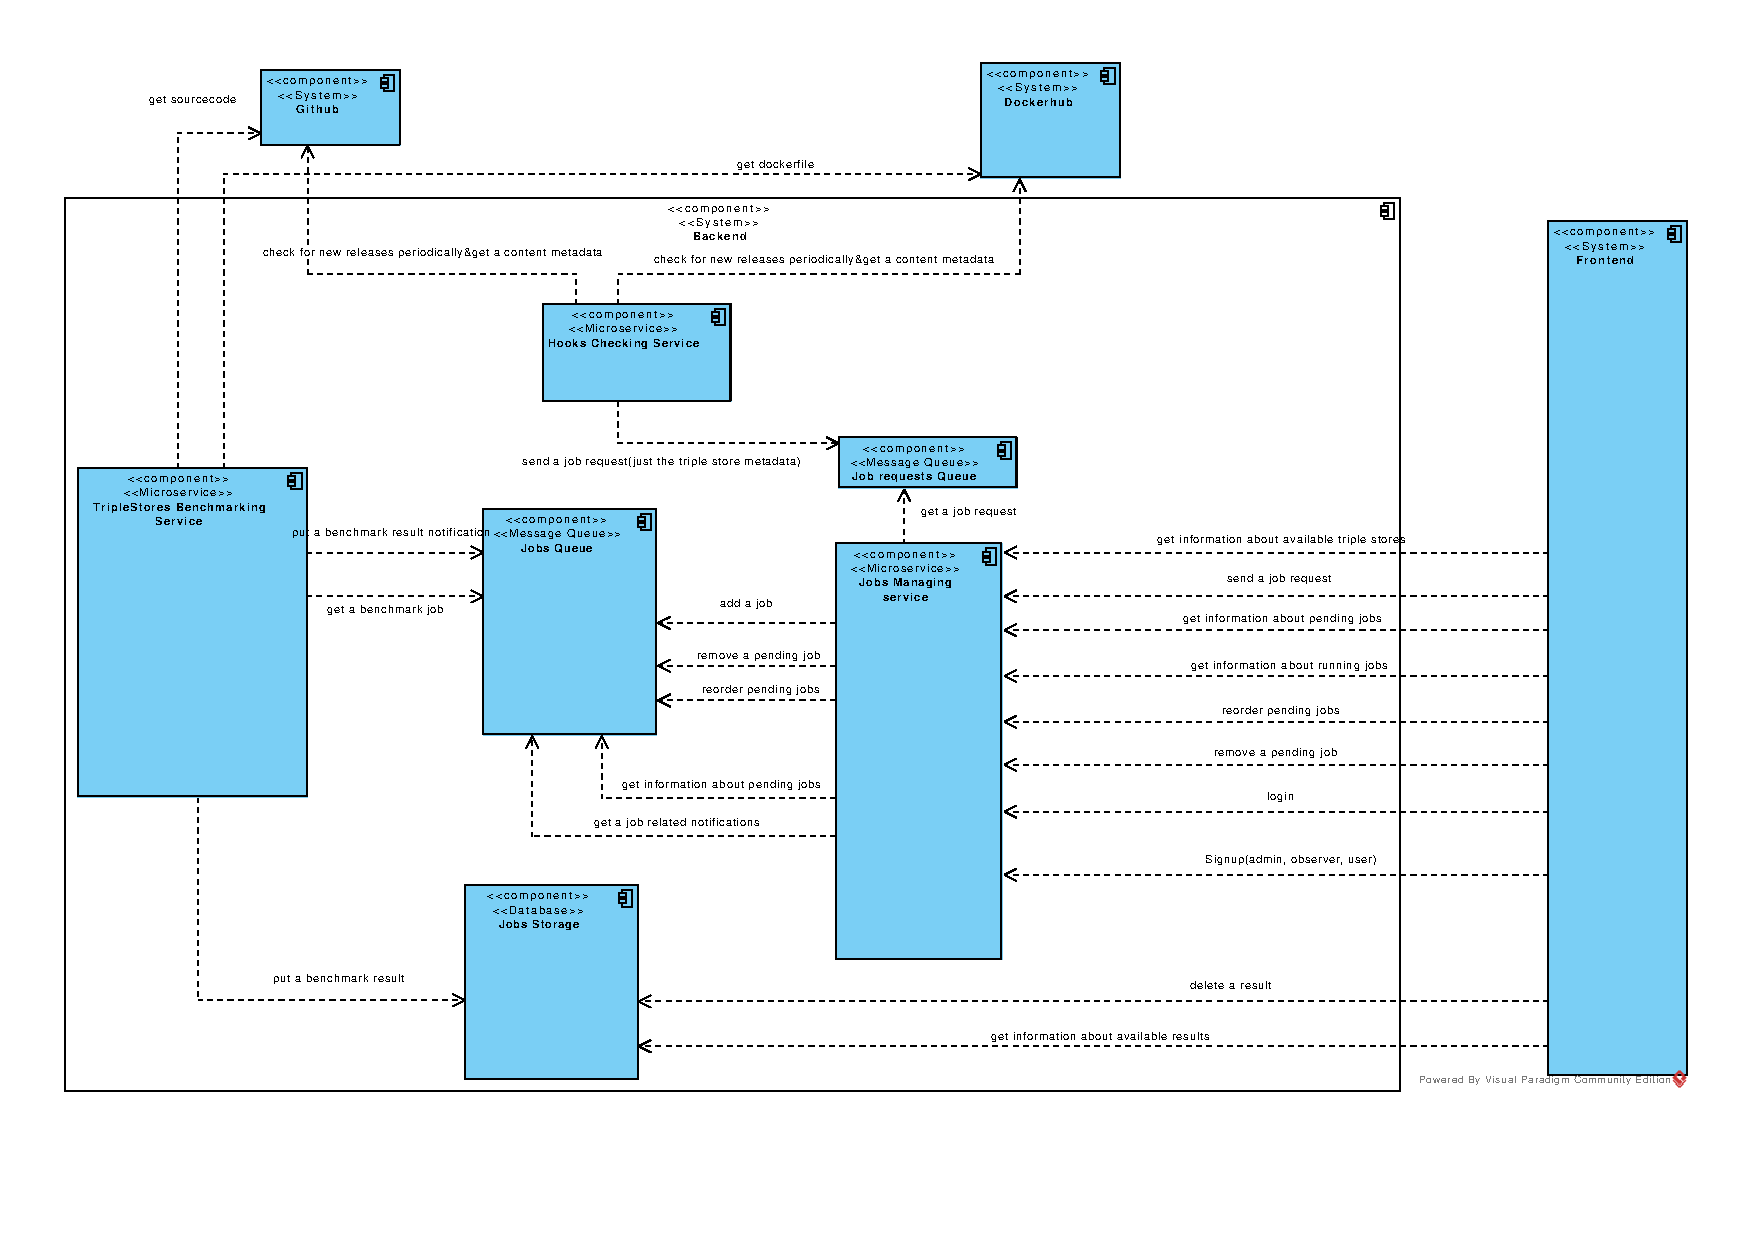
\includegraphics[width=1.1\textwidth]{figures/basilisk_high_level_design.pdf}
	\caption{High level design of the Basilisk framework}
	\label{fig:basilisk_high_level_design}
\end{figure}
\\

\section{Main Services}
\label{sec:main_services}
The next sections explain the three main services, namely \acl{hcs} (section \ref{sec:hooks_checking_service}), \acl{jms} (section \ref{sec:jobs_managing_service}), and \acl{tbs} (section \ref{sec:ts_benchmarking_service}).

This explanation follows the flow of actions that happen while configuring a continuous benchmark and the actions that happen when a benchmark is initiated.

The explanations are based on provided diagrams, code review and analysis, and information provided by former developers of the project.
\todo{okay to say this?}


\subsection{\acl{hcs}}
\label{sec:hooks_checking_service}
The main task of the \ac{hcs} is to observe \gh{} and \dockh{} repositories of \tsp{} for new releases or changes.

When a user wants to set up a new continuous benchmark, the \ac{hcs} needs to be informed which repository (\gh{} or \dockh{}) has to be observed for changes.
This happens through REST API calls to the \ac{hcs} providing the repository name and owner.
The \ac{hcs} will then create a hook for the repository to get notice about changes.
A hook is in general a piece of code or software that attaches itself to a software component to intercept messages and react to those messages, \eg, with function calls.
In the case of the \ac{hcs} the hooks can be seen as bookmarks for the repositories.
Each hook stores the latest known version of an repository.
The service will query the saved repositories regularly and compare their current version to the version stored in the hook.

When the \ac{hcs} notices a new release for a repository, it updates the corresponding hook to the newest version.
Then it sends a message about the new version to the \aclp{jrq} from which the \acl{jms} retrieves the message.

\subsubsection{API and Messaging}
\label{sec:hooks_api}
The \ac{hcs} is controlled by the user over a REST API.

The continuous checking of the repositories can be started and stopped over a REST endpoint.
The other most important endpoints are for adding and deleting \gh{} and \dockh{} repositories.
\\

The communication between the \ac{hcs} and the \acl{jms} is done over RabbitMQ messages, over the \aclp{jrq}.
The messages contain different events that can occur in the \ac{hcs}.
For example an event is send when adding or deleting a repository, or a new release is detected.


\subsection{\acl{jms}}
\label{sec:jobs_managing_service}
The main task for the \acf{jms} is to create benchmark jobs, when a new release was found by the \ac{hcs}.
Other important functionality of the \ac{jms} is the management of configurations needed for the benchmarks.
Lastly the \ac{jms} manages the status for running and pending jobs send to the \acl{tbs}.
\\

There are three configuration types needed.
First the platform needs the configuration for the \ts{}.
This configuration include for example the SPARQL endpoint as well as the user and password for the connection to the endpoint.
This is needed by the \iguana{} framework to properly connect to the \ts{} under test\cite{IguanaDocumentationConfiguration}.

Secondly the platform needs configurations for datasets and query configurations.
The dataset configuration simply consists of the dataset name and the URL for the location of the dataset.
The query configuration consists similarly of a name for the queries and the URL for the location of the query file.

These configurations are added over the REST API of the \ac{jms}.
\\

When the \ac{hcs} sends an event regarding a new release of a repository, the \ac{jms} will create benchmark jobs for the new release.
A benchmark job consists of the current version of the repository, a query configuration and a dataset.
For each event multiple benchmark jobs can be created.
For each query configuration and dataset one benchmark job will be created.

These benchmark jobs will then be send to the \acl{tbs} over the \acl{bjq}.

The management of the running and pending benchmark jobs is done over the REST API of the \ac{jms}.
When an endpoint is triggered, \eg, to abort a running job, the \ac{jms} sends an event to the \acl{tbs}.


\subsubsection{API and Messaging}
\label{sec:jobs_api}
The \ac{jms} communicates with the \ac{hcs} and the \acl{tbs} over message queues.
The service receives repository events from the \ac{hcs} and sends benchmark job events to the \acl{tbs} over the \ac{bjq}.
\\

Interaction of the user is handled over the REST API.
Over the API the different configurations can be added.

Currently the API is not yet implemented.
This will be done during the implementation phase of this thesis.
\todo[inline]{Here? or in \ref{sec:architecture_review} Review?}


\subsection{\acl{tbs}}
\label{sec:ts_benchmarking_service}
The \ac{tbs} executes the benchmark jobs send by the \ac{jms} and saves the benchmark results to a \ts{}.

To execute a benchmark the service needs a running instance of the \ts{} under test on which the benchmark will be executed.
This instance is build from the information and configurations provided in the benchmark job.
The \ac{tbs} will query the provided repository (\gh{} or \dockh{}) for the version, specified in the job.

If the repository is from \gh{}, the \ac{tbs} downloads the source code for the provided commit and looks for a Dockerfile.
It then builds and runs a Docker Container from that Dockerfile.

If the repository is from \dockh{}, the \ac{tbs} pulls the image with the provided tag.
It then runs the image as a Docker Container.

After starting the Docker Container the \ac{tbs} starts the \iguana{} framework.
\iguana{} will perform the benchmark with the provided configuration from the benchmark job.

When the benchmark is finished the results are written to a \ts{} called \acl*{jsts}

\subsubsection{API and Messaging}
\label{sec:benchmarking_api}
The \ac{tbs} has no REST API.
The service is controlled through the \ac{jms} by events send over RabbitMQ.

The events received from the \ac{jms} are new benchmark jobs and pause or abort commands for running benchmark jobs.
The \ac{tbs} sends short events containing the status of benchmark jobs, \eg, a job has started, or it has finished and the results are uploaded to the \acl{jsts}.



\section{Message Queue System}
\label{sec:message_queue}
The messages send between the services are transmitted via the RabbitMQ (\ref{sec:rabbitmq}) message broker.

There are two groups of queues.
The first group consists of the \aclp{jrq} through which the \ac{hcs} and \ac{jms} communicate.

The second group consists of the \aclp{bjq} through which the \ac{jms} and the \ac{tbs} communicate.



\section{Programming Language and Frameworks}
\label{sec:prog_lang_and_framework}
All services are implemented with Java and are using the Spring Boot framework.

The package structure used for the implementation of the services is similar in all three services.
It is strongly influence by the structure recommended for the Spring Boot framework.
The Spring and Spring Boot framework are shortly described in chapter \ref{sec:spring}.

\todo[inline]{Is this chapter needed? The queues are explained in API / Messaging sections of each service}


\section{Architecture Review}
\label{sec:architecture_review}
In this section we review the architecture three services of the Basilisk platform.
We point out possible problems with current implementations and list missing implementations that need to be added.

\todo[inline]{Not yet final.. only a first collection of thoughts and implementation todos}

\subsection{Management of Repositories and Configurations}
\label{sec:management_repo_config}
Currently the observed repositories are managed and stored in the \ac{hcs} while the configurations for the \tsp{} are managed and stored in the \ac{jms}.
This makes it difficult to connect a repository to a \ts{} configuration, since they are stored in different services.

The current implementations tries to solve this problem, by sending events about repository creations from the \ac{hcs} to the \ac{jms}.
This results in the duplication of the repository storage in both services.


\subsection{Missing Implementations}
The Basilisk platform is not yet fully implemented.
After reviewing the source code the following overview was created:

\subsubsection{\acl{hcs}}
The implementation of the \acl{hcs} is quite complete.
Only small additions have to be implemented.

\begin{itemize}
	\item The REST endpoints for deleting \gh{} and \dockh{} repositories needs to be added.
	
	\item Currently Pull Requests in \gh{} repositories can not be observed.
\end{itemize}


\subsubsection{\acl{jms}}
The implementation of the \acl{jms} is mainly missing the REST API and some internal logic.
The following REST endpoints have to be added:

\begin{itemize}
	\item Adding / removing \ts{} configurations
	
	\item Adding / removing dataset configurations
	
	\item Adding / removing query configurations
\end{itemize}

Since the \ac{jms} also manages the running and pending benchmark jobs, the REST API and internal logic for managing these jobs needs to be implemented too.

\begin{itemize}
	\item List running / pending jobs and their status
	
	\item Set the status for a job
\end{itemize}



\subsubsection{\acl{tbs}}
The implementation of the \acl{tbs} is currently only a bare structure.
Big parts of the logic needs to be implemented.

Currently the existing classes are mainly for storing configurations and basic message queue interactions.
These classes do not carry much functionality.

The main functionality needs to be implemented.
This consists of setting up the Docker containers which contain the \tsp{} for benchmarking:

\begin{itemize}
	\item Pulling Code from \gh{}
	\item Pulling images form \dockh{}
	
	\item building Docker containers from Dockerfiles / images
	
	\item connection to the Docker containers
\end{itemize}

Then the usage of the \iguana{} framework needs to be implemented.

Lastly, after the benchmark, some cleanup of the Docker containers needs to be implemented.


